\section{Light Capturing Devices}
This section deals with the basic evolution of light capturing devices.
\subsection{Notes}
Initially, there was a single cell 1D capture of light. This had many problems, but the main one being it can only capture light from one direction, and had no understanding of the intensity of it (binary). Using multiple 1D Cells allowed for more directions to be captured.
\begin{figure}[!htb]
	\center{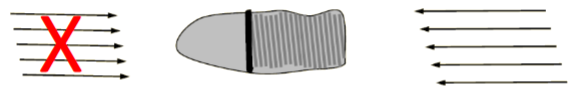
\includegraphics[width=10cm]
		{vision/1dcell}}
	\caption{\label{fig:1dcell} 1D Cell}
\end{figure}
Having multiple cells curved allowed for capture of light from various directions, somewhat conic. But it had difficulty keeping track of an image, as the same image would be hitting too many cells, so it would be all over the place.
\begin{figure}[!htb]
	\center{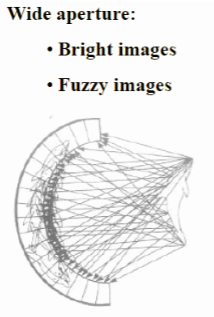
\includegraphics[width=4cm]
		{vision/wideaperture}}
	\caption{\label{fig:1dlinearcell} 1D Cell Curved Array}
\end{figure}
The concept of a pinhole camera was the next step, but there was an issue. With the wide aperture, the images were bright but they were fuzzy. With the pinhole, the images were sharp but they were too dim. How can we get the positives without the negatives?
\begin{figure}[!htb]
	\center{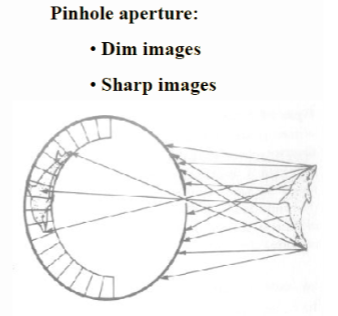
\includegraphics[width=4cm]
		{vision/pinholeaperture}}
	\caption{\label{fig:pinholeaperture} Pinhole}
\end{figure}
Simple, refraction from lenses. By having a lens refract light into the pinhole camera, or image point, it would allow for all the light to pass through the pinhole and hit different cells based on the initial angle the light hit the lens, maintaining the brightness from the wide aperture with the clarity of the pinhole aperture.

The virtual image created is upside down, and our eyes, based on this concept, simply allow the brain to flip it back.
\begin{figure}[!htb]
	\center{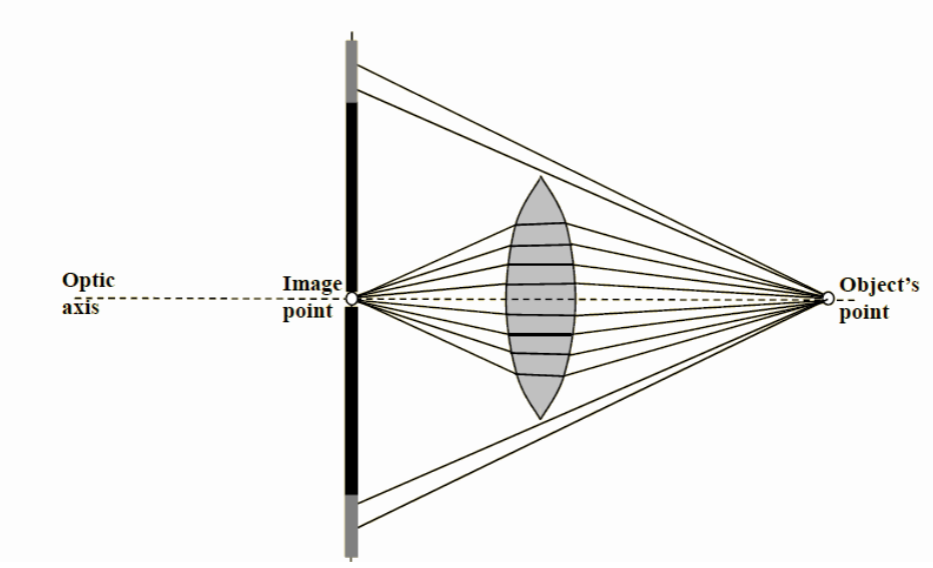
\includegraphics[width=5cm]
		{vision/lens}}
	\caption{\label{fig:lens} Lens in action}
\end{figure}
\section{Human Vision}
This section deals with human vision, a fairly straight forward topic (at least in our scope, this stuff can get wild pretty fast).
\subsection{Notes}
The human retina contains two types of photo receptor cells. Rods, of where there are ~120 million, and Cones, of which there are ~6 million. Rods are extremely sensitive to light and respond to single photons. They have poor spatial resolutions as multiple of them converge to the same neuron for data handling. However, thanks to their sensitivity, they help us see light in the dark.
This is different with cones, which are active at higher light levels. Several neurons process Cone data, so they have higher spatial resolution than rods.

\textbf{Receptive Field}

The receptive field is the area on which light must fall for neurons to be stimulated.The size of a receptive field determines a few things. Small receptive fields are stimulated by high spatial frequencies; and large spatial fields are stimulated by low spatial frequencies.  There are differences between the centre and periphery of field. We can't talk about these without talking about ganglion cells.
\begin{figure}[!htb]
	\center{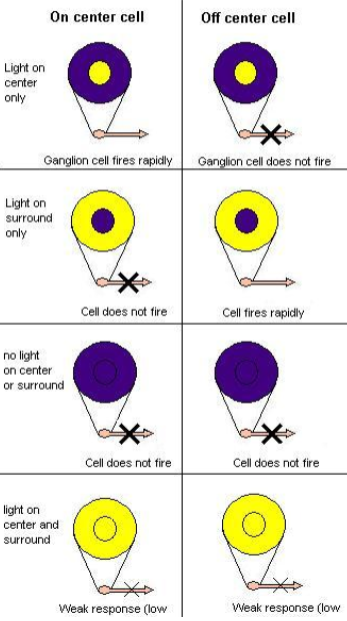
\includegraphics[width=6cm]
		{vision/ganglion}}
	\caption{\label{fig:lens} Ganglion responses}
\end{figure}
There are two types of ganglion cells, on-centre and off-centre, as seen in the image. On-centre cells are stimulated when the center is exposed to light, and are inhibited when the surrounded area is exposed. This works opposite for off-centre cells, as the name suggests.

Ganglion cells have a higher action potential rate depending on the intensity and location of light hit. This allows us to have a grasp at contrast, as it responds differently to different intensities of light.

\textbf{Visual Pathway}

\begin{enumerate}
	\item Vision generated by photoreceptors in the eyes (as explained above)
	\item The information leaves the eye by way of the optic nerve. Special note: The humans have a blind spot in the eye that does not allow them to see at one specific part of the eye; this is the optic nerve's location. Without it, we wouldn't be able to actually see.
	\item There is a partial crossing of axons at the optic chiasm; this allows the brain to receive data on the same visual field from both eyes, superimposing images, creating a sense of depth, etc.
	\item The axons following the chiasm, also known as the optic tract, wraps around the midbrain to get to the lateral geniculate nucleus (LGN).
	\item The LGN axons fan out to the deep white matter of the brain before ultimately travelling to the primary visual cortex at the back of the brain, where the magic happens.
\end{enumerate}
\begin{figure}[!htb]
	\center{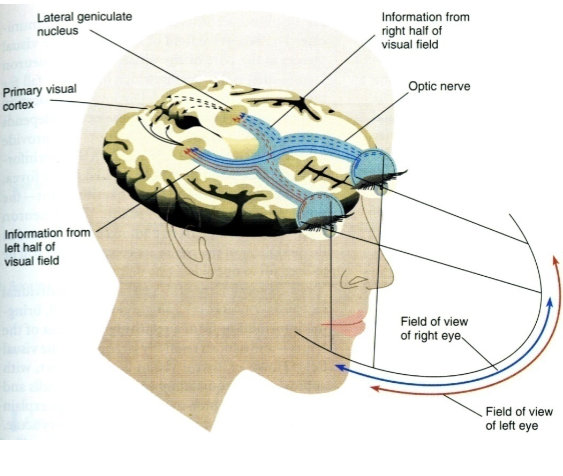
\includegraphics[width=5cm]
		{vision/visualpathway}}
	\caption{\label{fig:visPathway} Visualising the visual pathway}
\end{figure}

\section{Edge Detection}
\subsection{Convolving a Matrix}
\begin{figure}[!htb]
	\center{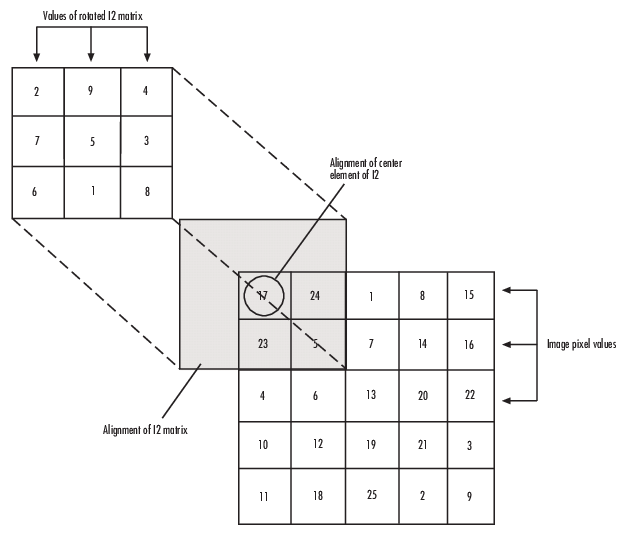
\includegraphics[width=9cm]
		{vision/convolve}}
	\caption{\label{fig:convolve} 3x3 convolution example}
\end{figure}
2D convolution of matrices is basically what the course is built off of, at least for edge detection. So its important to know how to do it. Given a 3x3 kernel and an MxN matrix, how does one convolve? Looking at the image, you will create a new matrix by overlaying the kernel with the matrix, multiplying each term on the kernel with the value it overlays and then sum them all up. The new generated value will then be placed in the same position as the centre of the overlay. 

\textbf{Note: for even kernels, you can select either the top-left or top-right centre value as the "centre" of the matrix.}

\subsection{First Order Operators}
Edge detection operators are approximation of the first order derivative of the colours. The change in intensity of the colour from a set of points. The gradient of the intensity of colours. I could explain it in mnay different ways, but basically since edges are generally a different shade from its background, checking for a larger change in the intensity would usually return an edge point.
\newline
The approximations take the form of different kernels. Small kernels usually don't give a good enough approximation, and using too large a kernel would just blur all the values together and miss edges.
\begin{enumerate}
	\item Sobel Operator: The sobel operator uses two kernels; one for the x-gradient and one fo the y-gradient. $G_x =
	\begin{bmatrix}
		-1 & 0 & +1 \\
		-2 & 0 & +2 \\
		-1 & 0 & +1
	\end{bmatrix}$ and $G_y = 
		\begin{bmatrix}
	-1 & -2 & -1 \\
	0 & 0 & 0 \\
	+1 & +2 & +1
	\end{bmatrix}$
	\item Roberts Operator: The roberts operator can also use two kernels, but it instead measures the change diagonally. $G_x =
	\begin{bmatrix}
	+1 & 0 \\
	0 & -1 \\
	\end{bmatrix}$ and $G_y = 
	\begin{bmatrix}
	0 & +1 \\
	-1 & 0 \\
	\end{bmatrix}$
\end{enumerate}

Once we have applied $G_x$ and $G_y$, and assuming we have a threshold $h$ (the threshold can be found either with trial and error or setting up some Ai to test with a control set); the final edge pixels can be generated with the approximation:
\begin{equation}
I = (h > \left| G_x \right|  + \left| G_y \right| )
\end{equation}

Edges generated like this might be susceptible to noise, because derivatives are looking for changes in the intensity. Noise are not part of the source, but rather a bi product from the limitation of our cameras and files. (JPG compressed image for example) When a derivative filter is used, it will simply return the change in intensity from the noise as part of the image. Depending on the quantity of noise, it could end up being a complete mess.

We can remove noise using the most common kernel, with the power of Gaussian. It is a gaussian distribution in the form of a 2D kernel, with the highest value in the centre of the matrix. The size of the matrix alters the effect of the noise filtering. A smaller matrix won't filter much, since it's not looking at a large enough space, and using too large a matrix will just blur the image together, removing edges.
\begin{figure}[!htb]
	\center{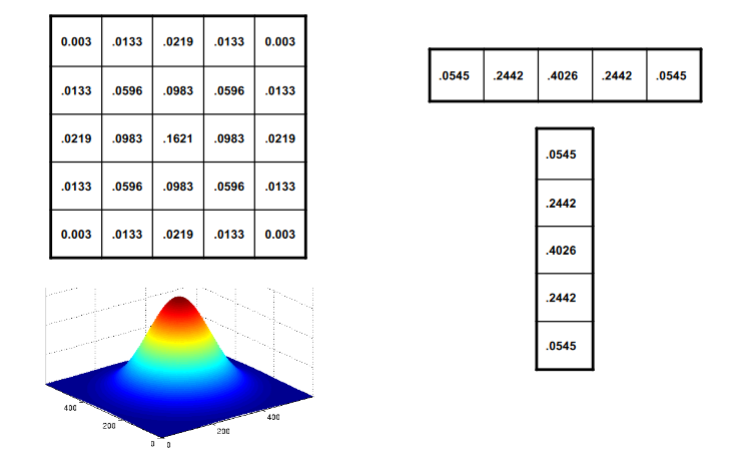
\includegraphics[width=9cm]
		{vision/noiseMat}}
	\caption{\label{fig:noiseMat}Gaussian Noise Filter overview}
\end{figure}

Rather than convolving the 2D Gaussian with the image, there is a more efficient way to go about this. You can create two 1D matrices $(1xn, nx1)$ and convolve those instead. The result will be the same, and it will be much faster than just doing the 2D matrix as there are less computations to deal with.

\subsection{Second Order Operators}
There is also the option of using Second Order Derivative operators. These function slightly different than first order, as seen in the image. 
Second Order Derivates look for the zero-crossings. These are the points the values of the graph change signs by crossing the 0-point of the axis. These points are the local maxima/minima in the first order operators. This method is very susceptible to noise, as noise will cause the function to cross zero many times. To alleviate these potential errors, we can apply a gaussian noise filter and a threshold for the distance needed to travel after crossing 0 to be counted as a "zero-crossing".
The second order operator, Laplacian Operator, can be derived as follows:
\begin{flalign}
	\begin{split}
	\frac{\partial^2 f}{\partial x^2} = &\frac{\partial G_x}{\partial x} \\
    = &\frac{\partial (f[i,j+1] - f[i,j])}{\partial x} \\
	= &\frac{\partial f[i,j+1]}{\partial x} - \frac{\partial f[i,j]}{\partial x} \\
	= & (f[i, j+2] - f[i, j+1]) - (f[i,j+1] - f[i, j]) \\
	= & f[i, j+2] - 2f[i,j+1] + f[i,j]
	\end{split}
\end{flalign}
The equation above is centred on $[i, j+1]$; if we want to centre it on $j$, we simply do $-1$ on all terms, and up with the following stuff.
\begin{flalign}
	\begin{split}
	\frac{\partial^2 f}{\partial x^2} = & f[i, j+1] - 2f[i,j] + f[i,j-1] \\
	\frac{\partial^2 f}{\partial y^2} = & f[i+1, j] - 2f[i,j] + f[i-1,j] \\
	\Delta^2 \approx & \begin{bmatrix}
	0 & 1 & 0 \\
	1 & -4 & 1 \\
	0 & 1 & 0
	\end{bmatrix}
	\end{split}
\end{flalign}

We can also place the equation inside of a gaussian distribution function, and end up with a Laplacian of Gaussian (LoG), a potentially efficient second order operator.

\subsection{Canny Edge Detection}
Our new friend and scientist, J. Canny, has shown that the first derivative of the Gaussian closely approximates the operator that optimizes the product of signal - to - noise ratio and localization.

Canny Edge Detection is sort of a standard (its pretty good). There are four major steps to canny edge detection.
\begin{enumerate}
	\item Find $f_x = f * G_x$ and $f_y = f * G_y$ where $G(x,y)$ is the gaussian function and $G_{x/y}$ is the derivative with respect to the required variable. $G_a = \frac{-a}{\sigma^2}(G(x,y))$
	\item Compute the gradient magnitude and direction.\[ mag(x,y) = \left| f_x \right| + \left| f_xy \right| \] \[dir(x,y) = \arctan{\frac{f_y}{f_x}}\]
	\item Apply non-maxima suppression. In simpler maths terms, check if the gradient magnitude at a pixel is a local maximum along the gradient direction.
	\item Apply hysteresis thresholding. This is fancy for applying a threshold at a low value $t_l$ and a high value $t_h$, which is usually twice $t_l$. First mark the edges generated from the high threshold, as these are strong edges and are generally genuine. Trace an edge with the bidirectional information and, while tracing, apply the lower threshold to trace faint sections of edges that have a start point.
\end{enumerate}


\subsection{References}
\href{http://fourier.eng.hmc.edu/e161/lectures/canny/node1.html}{Canny Edge Detection}

\href{https://pdfs.semanticscholar.org/d5c1/d380263318c1b7a7d298500b3617e55ef2fa.pdf}{A paper on Edge Detection}

\href{http://www.me.umn.edu/courses/me5286/vision/VisionNotes/2017/ME5286-Lecture7-2017-EdgeDetection2.pdf}{Good Lecture on Topic}

\section{Facial Recognition}
This section deals with the general idea of Facial Recognition.
\subsection{Eigenfaces}
Lets start by thinking of the face as a weighted combination of different components or representations of said face. These components are referred to as Eigenfaces (because who needs real words). Luckily, we can represent all these components as vectors. Eigenfaces are used in two ways; either as a form to store faces for later reconstruction or for recognition of a new image of a familiar face. We can do the learning using Principle Component Analysis (PCA).\newline
Given a set of points in 2D, as in the image, you can use vectors in the place of the usual line of best fit. When we use vectors, we would ideally want it to be in normal form with a scaling factor applied to it. This is where Eigenvectors come in. Eigenvectors take the following form: \[\boldmath{A}\vec{v} = \mu\vec{v}\] where $\mu$ is referred to as the "eigenvalue". Eigenvectors are obtained from a matrix, and follow some rules.
\begin{itemize}
	\item Only square matrices have eigenvectors
	\item Different matrices have different eigenvectors
	\item Not all square matrices have eigenvectors
	\item An $n \times n$ matrix has at most $n$ distinct eigenvectors
	\item All distinct eigenvectors of a matrix are orthogonal
\end{itemize}
You ask, where do we get the matrix in this instance? We do it by finding a covariance matrix. Since we have a 2D plot of points, we can generate a 2x2 covariance matrix. This can be done by the following equations, the first for the covariance matrix, and the other for the variance function.
\[	C = \begin{bmatrix}
Var(x_1) & Covar(x_1, x_2) \\
Covar(x_1,x_2) & Var(x_2)
\end{bmatrix}\]
\[ Covar(x_1, x_2) = \frac{\sum_{i=1}^{n}(x_1^i - \bar{x_1})(x_2^i - \bar{x_2})}{n-1}\]
With faces, we treat the face as a point in a high-dimensional space, and then treat the training set of faces as our set of points. We calculate the eigenvectors of our training set, and these become our eigenfaces. \textbf{TL;DR Eigenfaces are eigenvectors of covariance matrix of training set of faces}\newline
When given an image of a face, we can transform it into face space (Facebook?) by applying the following equation: \[w_k = x^i\vec(v_k)\] where $k$ is the number of eigenfaces, with the $i^{th}$ face in image space, and a corresponding weight $w$. Image recognition becomes easy, simply find the euclidean distance of the desired face and all faces stored; the closest face is most likely our match. You can also reconstruct a face from the eigenfaces. The more eigenfaces the better the reconstruction.
\subsection{References}
Just the slides
\section{Vision Systems}
This section deals with feature detection of vision systems.
\subsection{Invariants}
Ideally, we would like some invariance in different settings for what we would like to see.
\begin{enumerate}
	\item Illumination: Can be achieved by normalising the light levels and storing the new normal intensities. Can also used difference based metrics (sift).
	\item Scaling: Store pyramids of the image, with each step half the size of the original. Find pixel values with Gaussian blur. Can also use Scale Space method, using Difference Gaussians to find repeatable points (invariant) in scale.
	\item Rotation: Rotate all features to go the same way in a determined manner. Take histogram of gradient directions and rotate to the most dominant.
\end{enumerate}
\subsection{Feature Detection}
In motion tracking, our goal is to see things that move between a set of images. You can begin by knowing which of the four following cases fits best:
\begin{enumerate}
	\item Stationary Camera, Stationary Objects
	\item Stationary Camera, Moving Object
	\item Moving Camera, Stationary Objects
	\item Moving Camera, Moving Object
\end{enumerate}
When detecting change, you can compare the intensity at one point in time with its previous incarnation (or any other, if you need something specific). However, this lends to issues appearing from random noise, which will pop up everywhere. What we want is to then filter out our noise, but how do we do such a thing?

We can use the idea of 8 or 4 connectedness. Two pixels are 4-neighbours if they share an edge, and are 8-nieghbours if they share a corner. Two pixels are 8-connected if we can create a path of 8-neighbours from one to another. We can use these concepts and group pixels into clusters. We can then threshold the clusters and remove any clusters that are below said threshold, ideally leaving behind just the changes and removing noise.
\begin{figure}[!htb]
	\center{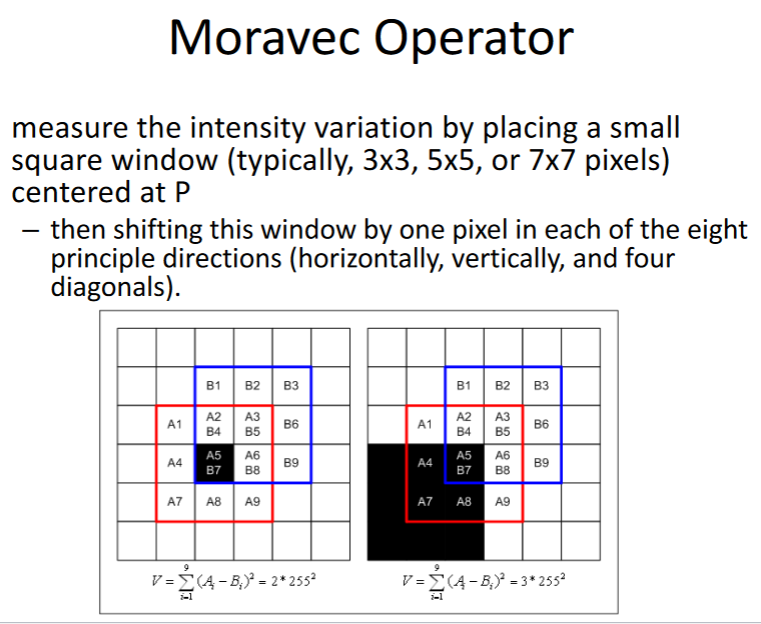
\includegraphics[width=9cm]
		{vision/moravec}}
	\caption{\label{fig:moravec}Gaussian Noise Filter overview}
\end{figure}
However, just seeing the difference in pixels might not be enough. Ideally, we would want to find our points of interest and compare those points between images. For this, we can use the Moravec operators, a corner detector. Corners are better than edges for this task because corners can measure the highest intensity change, as oppose to edges. The image explains how the Moravec operators works. Once we obtain our new values from our friend Moravec, we can just keep the local maxima.\newline

Motion Correspondence has three main principles we need to worry about.
\begin{enumerate}
	\item Discreteness: Measure of the distinctiveness of individual points
	\item Similarity: Measure of how closely two points resemble one another
	\item Consistency: Measure of how well a match conforms with nearby matches
\end{enumerate}
\subsection{Object Detection}
Object recognition needs the following components:
\begin{enumerate}
	\item Model Database: Stores all models known by the system; information stored depending on approach for recognition. Generally, these values are abstract (shape, colour, size, etc.)
	\item Feature Detector: Applies operators to image and identifies location of features. How a feature detector works depends on what types of models are stored in the database.
	\item Hypothesizer: Assigns likelihoods to objects present to reduce computational expense.
	\item Hypothesis Verifier: Uses object models to verify hypothesis and refines the hypothesizer likelihood. 
\end{enumerate}
Each of these components come with issues, mostly related to what sort of thing you want to do. (2D vs 3D, model vs object, etc.)